\documentclass[tikz,border=8pt]{standalone}
\usepackage{amsmath,amssymb}
\usetikzlibrary{arrows.meta,calc,decorations.markings}

\begin{document}
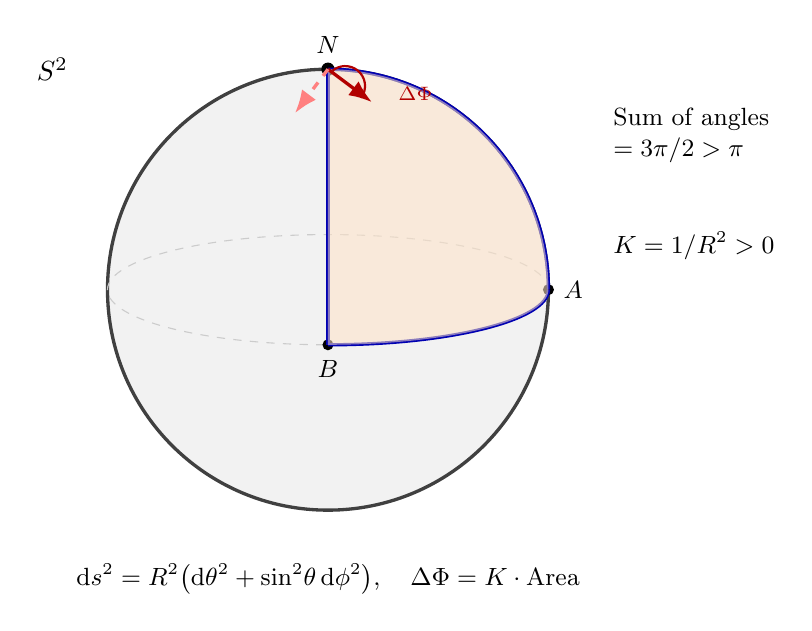
\begin{tikzpicture}[>=Latex, scale=1.4]

  % Sphere
  \draw[very thick, gray!50!black, fill=gray!10] (0, 0) circle (2.0);
  \draw[gray!40, thin, dashed] (0, 0) ellipse (2.0 and 0.5);

  % North pole
  \fill[black] (0, 2.0) circle (0.06);
  \node[font=\small, anchor=south] at (0, 2.05) {$N$};

  % Two equator points (90 deg apart visually)
  \fill[black] (2.0, 0) circle (0.05);
  \node[font=\small, anchor=west] at (2.05, 0) {$A$};
  \fill[black] (0, -0.5) circle (0.05);
  \node[font=\small, anchor=north] at (0, -0.55) {$B$};

  % Three sides of triangle (great-circle arcs)
  \draw[very thick, blue!70!black] (0, 2.0) arc (90:0:2.0 and 2.0);
  \draw[very thick, blue!70!black] (0, 2.0) .. controls (0, 1) and (0, 0) .. (0, -0.5);
  \draw[very thick, blue!70!black] (2.0, 0) arc (0:-90:2.0 and 0.5);

  % Shade triangle
  \fill[orange!22, opacity=0.55]
    (0, 2.0) arc (90:0:2.0 and 2.0) arc (0:-90:2.0 and 0.5) .. controls (0, 0) and (0, 1) .. (0, 2.0) -- cycle;

  % Parallel transport: vector at N (start) and after going around (rotated 90)
  \draw[->, very thick, red!70!black] (0, 2.0) -- (0.4, 1.7);
  \draw[->, very thick, red!50, dashed] (0, 2.0) -- (-0.3, 1.6);

  % rotation arc (delta phi)
  \draw[red!70!black, thick] (0.30, 1.74) arc (-37:130:0.18);
  \node[font=\scriptsize, red!70!black, anchor=west] at (0.55, 1.78) {$\Delta\Phi$};

  % Side text labels
  \node[font=\small, anchor=west, align=left] at (2.5, 1.4) {Sum of angles\\$=3\pi/2 > \pi$};
  \node[font=\small, anchor=west] at (2.5, 0.4) {$K = 1/R^2 > 0$};

  % S^2 label
  \node[font=\bfseries] at (-2.5, 2.0) {$S^2$};

  % Bottom formulas
  \node[font=\small, anchor=north] at (0, -2.4)
    {$\mathrm ds^2 = R^2\bigl(\mathrm d\theta^2+\sin^2\!\theta\,\mathrm d\phi^2\bigr),\quad \Delta\Phi = K\cdot\mathrm{Area}$};
\end{tikzpicture}
\end{document}
